\chapter{La Testing Factory}

La Testing Factory est un service chargé de réaliser la recette d'un projet. C'est à dire la phase pendant laquelle les différents acteurs du projet vérifient que le produit est conforme au cahier des charges et aux attentes du client. Il s'agit donc principalement de tests d'intégration fonctionnels, dont le périmètre est conçu par la testing et validé par le client, mais aussi de tests de non-régression permettant de vérifier que l'intégrité d'une application n'est pas affectée par une évolution.
Le but des testeurs n'est pas uniquement de valider ou pas une évolution, ils doivent également d'avoir une connaissance pointue des applications sur lesquelles ils travaillent, pouvant ainsi avoir un point de vue critique sur les applications et donc de concevoir des périmètres de tests plus pertinents.

Ces tests interviennent juste avant la phase de production, les testeurs n'ont donc pas le droit à l'erreur et doivent suivre des protocoles très stricts. Pour arriver à un haut niveau de qualité, la Testing Factory utilise la méthodologie TestFrame.

La Testing Factory Logica prend en charge les tests d’intégration fonctionnelle des applications de La Banque Postale composées des principaux domaines suivants :
\begin{itemize}
\item[$\bullet$] OASIS / SAFIR, qui regroupe la gestion des systèmes d’information concernant tous les processus métiers environnant les comptes dépôts et épargne.
\item[$\bullet$] SBMM / E-BNK / EPA BEL], qui regroupe la partie fonctionnelle du site de la Banque En Ligne (SBMM pour les particuliers et E-BNK pour les entreprises) et tous les types d’opérations (EPA BEL: virements, prélèvements, etc.…).
\item[$\bullet$] RSK, qui représente la partie de gestion des risques financiers liés aux transactions.
\item[$\bullet$] Référentiels / AE FAC], qui regroupe la partie Référentiel qui stocke tous les contrats (particuliers et entreprises) et AE FAC (Activité Entreprise FACturation) qui restitue les équipements des entreprises aux Centres Régionaux des Services Financiers (CRSF).
\item[$\bullet$] Média, qui regroupe toutes les applications iPhone et Android ainsi que le standard téléphonique 3639.
\item[$\bullet$] Automate qui développe le projet d’automatisation des tests.
\end{itemize}

Mais elle effectue également, pour ce client, des tests d’assemblage ou, encore, des tests de non régression. De plus, elle s’emploie également à diversifier ses activités avec des clients tels que Cdiscount, EDF, Cofinoga ou encore à répondre à des appels d’offre pour d’autres services de tests de Logica en France pour des clients comme France Telecom, Airbus, etc…


\section{Positionnement de la Testing Factory au cours d'un projet}

\begin{figure}[h]
  \begin{center}
    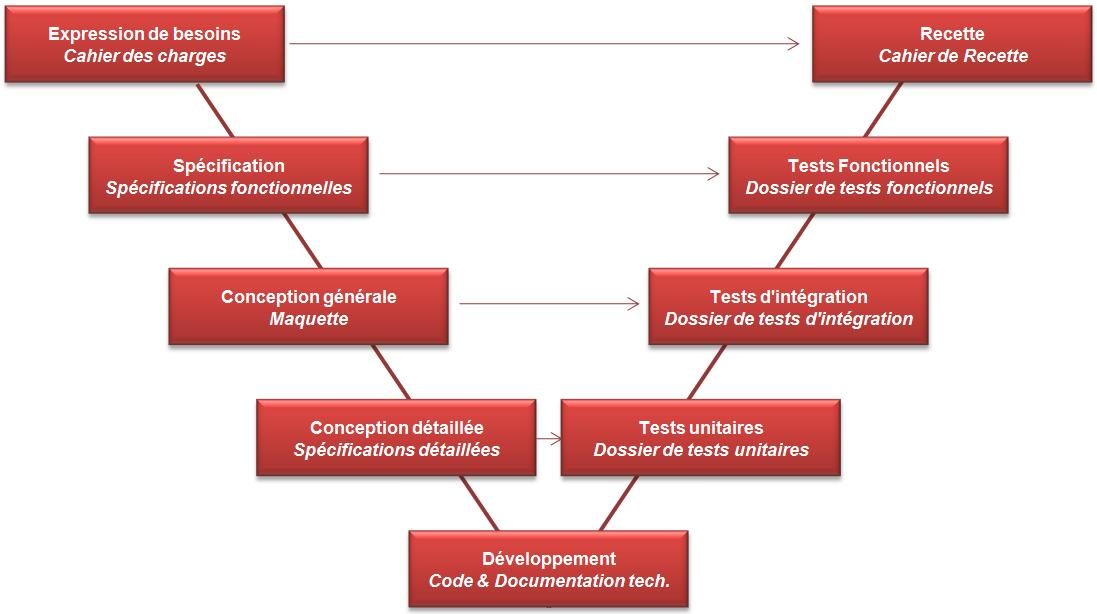
\includegraphics[width=15cm]{Images/Cycle_en_V.jpg}
  \end{center}
  \caption{Cycle en V d'un projet}
  \label{Cycle en V d'un projet}
\end{figure}

La testing factory se trouve à la fin du cycle d'un projet. Elle se charge d'effectuer les tests d'intégrations, les tests fonctionnels, et la recette du projet.
Pour chaque étape, le testeur dispose de documents de réference:
\begin{itemize}
\item Le dossier de conception générale pour les tests d'Integration.
\item Le dossier d'éxigences et de spécification pour les tests de validation.
\item Le dossier d'exigences pour la recette.
\end{itemize}

Ces différentes étapes sont importantes et l'ordre (test unitaire $\rightarrow$ test intégration $\rightarrow$ recettes) doit être respecté. En effet, faire les tests d'intégration avant les tests unitaires n'aurait pas de sens.
\clearpage
\section{Déroulement d'une phase de test}

\begin{figure}[h]
  \begin{center}
    \includegraphics[width=15cm]{Images/phase_de_test.png}
  \end{center}
  \caption{Déroulement d'une phase de test}
  \label{Déroulement d'une phase de test}
\end{figure}

\subsubsection*{ORGANISER - LE PTRMOE}
Le PTRMOE est le Protocole de Test et Recette MOE qui est conçu conjointement entre le RPMOE (Responsable de Projet MOE) et l’équipe de TI MOE afin de définir les modalités organisationnelles et opérationnelles de l’ensemble des étapes de tests du projet.
Il définit l’ensemble des fonctionnalités à évaluer, il évalue les risques et contraintes, il identifie les étapes à mettre en place, il organise et planifie l’activité de test et recette (T\&R). 
 
\subsubsection*{DEFINIR – Du plan de test au devis}
A partir du PTRMOE, et de documents de référence (cas d’utilisation, dossier de conception), l’équipe de TI MOE définit un périmètre de tests et élabore une liste de cas de tests ainsi que les jeux de données nécessaires pour couvrir le périmètre.
Les devis sont ensuite établis à partir d’abaques permettant de définir les charges (en jour/homme) que représente chaque étape d’une phase de test.
Une fois le devis établi, il peut être accepté tel quel par le RPMOE (débute alors la phase de conception) ou être rejeté (ce qui entraine une réévaluation du périmètre).

\subsubsection*{CONCEVOIR – Conception du cahier de test}
La phase de conception du cahier de test consiste à concevoir les cas de tests correspondant aux scenarii compris dans le devis retenu par le client. Ces cas de tests sont rédigés dans le cahier de test (qui est un fichier Excel) et sont regroupés par cas d’utilisation (Concept UML décrivant une fonctionnalité d’un système, quel qu’il soit).  Au sein de chaque cas d’utilisation, les scénarii sont construits et ordonnés en trois groupes :
\begin{itemize}
\item Les scénarii nominaux correspondant au comportement "normal" et attendu de la fonction testée.
\item Les scénarii alternatifs décrivant les cas plus complexes.
\item Les scénarii d’exception qui regroupent en général les cas d’erreurs.
\end{itemize}
La description d’un scénario de test doit être simple, claire et détaillée afin que n’importe quel testeur puisse l’exécuter sans aucune ambiguïté. 

\subsubsection*{REALISER - Déroulement des tests}
La phase d’exécution des cas de tests consiste à dérouler les cas de tests en suivant les scénarii établis au préalable, observer le comportement de l’application (il faut analyser les éventuelles anomalies rencontrées pour aider à leur qualification et non les déboguer), rédiger les rapports d’anomalies, tenir le cahier de test à jour (en y inscrivant événements et résultats), remonter les anomalies en les inscrivant dans l’outil de test et recette CARS.
Cette phase comprend aussi l’élaboration des jeux d’essais (données de tests) qui vont permettre la bonne exécution des scénarii de test. L’état d’exécution d’un cas de test est renseigné avec sigles:
\begin{itemize}
\item OK: Le test s’est déroulé correctement (il peut y avoir une preuve du bon fonctionnement avec des copies d’écrans par exemple)
\item Conception KO: La conception du cas de test est erronée et le scénario n’est pas déroulable
\item NE: Le cas de test n’est pas exécutable
\item NJ: Le scénario n’a pas encore été exécuté.
\end{itemize}

\subsubsection*{EXECUTER – Gestion des anomalies}
La gestion des anomalies est assurée par l’outil de test et recette CARS PORTAL (Compuware), c’est un outil de type workflow ou processus d’affaires permettant un flux d’information au sein d’une organisation. La gestion des anomalies mettant en jeu plusieurs acteurs: le testeur, le client, le développeur… cet outil permet une bonne communication sur l’évolution des anomalies.
On entend par anomalie de tests, tout dysfonctionnement de l’application qui, soit empêche l’utilisation de l’application, soit provoque un résultat ou une action incorrecte, alors que le logiciel est utilisé conformément à son objet (non-conformité de l’application par rapport à ce qui était convenu).
Tous les dysfonctionnements constatés lors d’une étape de tests sont consignés et référencés (numérotation séquentielle) dans des fiches d’anomalies classées selon leur niveau de gravité. Dans le but de favoriser l’efficience des tests, il est primordial que les fiches d’anomalies soient complètes, précises et se réfèrent à une trace.

\subsubsection*{EVALUER – Clôture des tests et bilan}
Les critères de fin d’exécution sont précisés dans le PTRMOE, sauf exception ils reprennent comme critères:
\begin{itemize}
\item Toutes les anomalies bloquantes doivent être clôturées.
\item Toutes les anomalies majeures portant sur au moins un scénario de tests de niveau de criticité "élevé" sont clôturées.
\item 100\% des scénarii de tests de niveau de criticité "très élevé" ou "élevé" sont exécutés avec un statut OK.
\item 80\% des scénarii de tests de niveau de criticité "moyen" sont exécutés avec un statut OK.
\end{itemize}

La phase de clôture des tests d’intégration se traduit par la rédaction d’un bilan. Le procès verbal de validation de l’étape de test est ensuite soumis au RPMOE pour signature.
Il peut arriver de façon exceptionnelle qu’une recette soit stoppée par décision du RPMOE (pour cause de trop grand nombre d’anomalies par exemple).

\section{TestFrame}

La méthode TestFrame a été développée par Logica pour produire rapidement des tests standardisés et rapide à concevoir.

\begin{figure}[h]
  \begin{center}
    \includegraphics{Images/diagramme_des_methodes.jpg}
  \end{center}
  \caption{Le diagramme des méthodes utilisée dans le processus de test}
  \label{Le diagramme des méthodes utilisée dans le processus de test}
\end{figure}
\subsection{Le dictionnaire des mots d'action}
Cette méthode s'appuie sur un dictionnaire de mot d'action répertoriant toutes les actions pouvant être effectuées par l'utilisateur sur une application sur chacun de ses écrans (appelés point pivots dans la méthodologie).
Chaque mot d'action est créé sur le modèle suivant et respecte un certain nombre de conventions:

\begin{figure}[h]
  \begin{center}
    \includegraphics[width=15cm]{Images/mot_action.jpg}
  \end{center}
  \caption{Patron d'un mot d'action}
  \label{Patron d'un mot d'action}
\end{figure}

Les mots d'action doivent respecter ces conventions:
\begin{itemize}
\item la première lettre de chaque mot doit être une majuscule.
\item pas d'accent dans les mots d'action.
\item on retire les mots d'action.
\item Un mot d'action ne doit pas contenir d'espace.
\item le verbe d'action doit faire partie de la liste des verbes autorisés (il y en a une douzaine en tout).
\end{itemize}

Exemple:\begin{bf}PopupEcranAccueil\_Cliquer\_OK\end{bf} conviendra pour l'action de cliquer sur le bouton "OK" de la popup apparaissant sur l'écran d'accueil.

Chaque mot d'action possède une description précise, ce qui permet de pallier un éventuel manque de précision. La structure de ce dictionnaire fait qu'il est très facile à mettre à jour en cas d'évolution de l'application, que ce soit pour modifier des mots d'action, en ajouter, ou en retirer. Par ailleurs, de très nombreux mots d'action sont réutilisables sur d'autres applications. Ce qui permet de rentabiliser le cout de l'élaboration du dictionnaire. En outre c'est cette structure qui permet de facilement automatiser les tests.

Une fois que le dictionnaire des mots d'action est terminé, l'élaboration de cas de test se simplifie car il suffit de mettre bout à bout les mots d'action pour effectuer un test.

\section{Automatisation des tests}

Certains projets bénéficie d'un automate de test, permettant d'executer des tests de non-régression. Pour cela, nous utilisons le progiciel TestPartner, qui nous permet de simuler une utilisation de l'application.
Chaque mot d'action de l'application est ainsi transformé en une fonction développée en Visual Basics (VB). Le coût de départ est assez élevé car il faut compter en moyenne un jour/homme par mot d'action, pour le développement et le test de chaque mot d'action. Cependant lorsque l'on considère que le partenariat avec la Testing Factory dure plusieurs années, on se rend compte que ce coût est rapidement rentabilisé.

Une fois que chaque mot d'action possède son équivalent en VB, des macros récupèrent les tests conçus grâce a TestFrame et créent les scripts à lancer dans TestPartner. C'est rapide et la base est la même que pour les tests manuels.

\subsection{Utilisation de TestPartner}

TestPartner est un outil essentiel du Pôle automate de la Testing Factory. C'est lui qui permet de faire le lien entre des éléments de l'application (bouton, lien, titre...) et la fonction associée au mot d'action.
\begin{figure}[h]
  \begin{center}
    \includegraphics[width=15cm]{Images/Bibliotheque_Mot_action_SAFIR.jpg}
  \end{center}
  \caption{Exemple d'une bibliothèque de SAFIRv1}
  \label{Exemple d'une bibliothèque de SAFIRv1}
\end{figure}

TestPartner est en fait capabable de de reconnaître les éléments d'une pages HTML qui ont été identifiés. Il se base pour cela sur les balises de la pages et sur une base de donnée crée par l'utilisateur. Il va donc pouvoir agir sur ces éléments (par exemple en écrivant dans un champs, en cochant une Checkbox, etc...). Cela demande tout de même que l'application testée soit codée proprement, car l'application se base sur les caractéristiques de chaque objet (type, taille, identifiant...).Si jamais certains éléments ne sont pas assez différenciés (par exemple s'il ne possède pas d'identifiant précis), TestPartner peut alors se tromper d'objet et estimer qu'il y a un bug et que le test est faux. A l'inverse, être trop précis sur les identifiants d'un objet peut empêcher TestPartner de le trouver. 
\clearpage
\begin{figure}[h]
  \begin{center}
    \includegraphics[width=15cm]{Images/capture_TestPartner_identifier.jpg}
    \caption{Capture d'un champs avec TestPartner}
    \label{Capture d'un champs avec TestPartner}
  \end{center}
\end{figure}


Le gros avantage de passer par un automate, c'est que les TNR vont pouvoir être éxecutés à chaque campagne de test. 
Lorsqu'un au automate est lancé, il va dérouler tout les cas programmé et va écrire dans une log le résultat de chaque mot d'action. une fois l'automate terminé, TestPartner retourne un rapport: 


\begin{figure}[h]
  \begin{center}
    \includegraphics[width=10cm]{Images/rapport_TestPartner.jpg}
    \caption{Exemple d'un rapport de tes partner}
    \label{Exemple d'un rapport de tes partner}
  \end{center}
\end{figure}


%\begin{figure}
%  \begin{small}
%    \begin{center}
%      
%\begin{verbatim}
%
%+++++++++++++++++++++++++++++++++++++++++++++++++++++++++++++++++++++++++++++++++++++++
%Public Function DOAdresseSpecifique_Verifier_BandeauTitreProcessusBandeau() As Boolean
%+++++++++++++++++++++++++++++++++++++++++++++++++++++++++++++++++++++++++++++++++++++++
%'Verifier le titre processus du bandeau  : doit être valorise  à ''Saisie d'une demande d'ouverture Epargne "
%
%On Error GoTo gesterr
%
%    Dim MyText As String
%
%    If Attente_Objet("IEWindow", "_IEWindow_InternetExplorer", "DOAdresseSpecifique") = False Then GoTo gesterr
%    If Attente_Objet("HTMLBrowser", "_HTMLBrowser_CadrePrincipal", "DOAdresseSpecifique") = False Then GoTo gesterr
%    
%    If Attente_Objet("HTMLDiv", "DOAdresseSpecifique_Libelle_BandeauTitreProcessus", "DOAdresseSpecifique") = False Then GoTo gesterr
%    MyText = HTMLDiv("DOAdresseSpecifique_Libelle_BandeauTitreProcessus").InnerText
%    If InStr(MyText, "Saisie d'une demande d'ouverture Epargne ") = 0 Then
%        Err.Description = "Le titre processus du bandeau n'est pas correct;Attendu : Saisie d'une demande d'ouverture Epargne ;Obtenu : " & HTMLBrowser("_HTMLBrowser%_CadrePrincipal").CaptureText
%        GoTo gesterr
%    End If
%    
%    DOAdresseSpecifique_Verifier_BandeauTitreProcessusBandeau = True
%        
%    'Ecrit dans log Fin OK
%    Call EcritDansLogMotDaction(fichierLog, "OK", "DOAdresseSpecifique_Verifier_BandeauTitreProcessusBandeau")
%    
%    Exit Function
%
%gesterr:
%    DOAdresseSpecifique_Verifier_BandeauTitreProcessusBandeau = False
%    'Ecrit dans log Fin KO
%    Call EcritDansLogMotDaction(fichierLog, "KO", "DOAdresseSpecifique_Verifier_BandeauTitreProcessusBandeau")
%End Function
%\end{verbatim}
%    \end{center}
%  \end{small}
%\end{figure}

